\documentclass[12pt]{article}


\usepackage[english]{babel}

% Set page size and margins
% Replace `letterpaper' with `a4paper' for UK/EU standard size
\usepackage[a4paper,top=2cm,bottom=2cm,left=3cm,right=3cm,marginparwidth=1.75cm]{geometry}

\usepackage[dvipsnames]{xcolor}
\definecolor{myblue}{RGB}{74, 144, 226}
\definecolor{myred}{RGB}{255, 2, 27}
%%%%%%%%%%%%%% Packages %%%%%%%%%%%%%%%%
\newtheorem{lemma}{Lemma}
%\usepackage{hyperref}
%\usepackage[...]{hyperref}
%\usepackage[colorlinks=true, allcolors=blue]{hyperref}
\usepackage[english]{babel}
\usepackage{amssymb}
\usepackage{underscore}
\usepackage{graphicx}
\usepackage{empheq}
\usepackage{booktabs}
\usepackage{tikz}
\newcommand*{\vertbar}{\rule[-1ex]{0.5pt}{2.5ex}}
\newcommand*{\horzbar}{\rule[.5ex]{2.5ex}{0.5pt}}
%% Some imports:
%\let\proof\relax
%\let\endproof\relax
%\let\example\relax
%\let\endexample\relax

%\usepackage{import}
\usepackage{float}
\usepackage{multirow}
\usepackage{amsmath}
% ,amsfonts,amssymb,amsthm
%\usepackage{subfigure}

\usepackage[ruled]{algorithm2e}
\usepackage{mathtools}
\usepackage[super]{nth}
\usepackage{caption}
\usepackage{subcaption}
\usepackage{graphicx}
%\usepackage{wrapfig}
\usepackage{verbatim} % comments
%\usepackage{comment}
%\renewenvironment{comment}{}{}
\usepackage{array}
\usepackage{supertabular}
\usepackage{longtable}
\usepackage{tabularx}
\usepackage{multirow}
\usepackage{colortbl}
\usepackage{fancyhdr}
%\usepackage{tcolorbox}
%\usepackage{tikz}
%\usetikzlibrary{math} %needed tikz library
%\usepackage[linesnumbered,ruled]{algorithm2e}
%\usepackage{pgf}
%\usepackage{pgfplots, pgfplotstable}
%\usetikzlibrary{fit,calc,positioning,decorations.pathreplacing,matrix}
%\usetikzlibrary{arrows}
%\usetikzlibrary{shapes}
%\usetikzlibrary{chains}
% Vector Styles
%\tikzstyle{load}   = [ultra thick,-latex]
%\tikzstyle{stress} = [-latex]
%\tikzstyle{dim}    = [latex-latex]
%\tikzstyle{axis}   = [-latex,black]
%\usepackage{pgffor}

%\usepackage{multido}
%\usepackage{calc}
%\usepackage{fp}
%\usepackage{xifthen}
%\usepackage{xargs}
\usepackage{etoolbox}
\DeclareMathAlphabet{\mathpzc}{OT1}{pzc}{m}{it}
\usepackage{breakcites} 
\usepackage[utf8]{inputenc}
\usepackage{helvet}
%\usepackage{geometry}
%\geometry{left=16mm, top=30mm, right=16mm, bottom=30mm}

%\usepackage{amssymb}
\usepackage{enumitem}
\usepackage{tabularx}
%\usepackage{xcolor}
\usepackage[absolute,overlay]{textpos}
%\usepackage{graphicx}
\usepackage{lipsum}
%\usepackage{caption}
\usepackage{multicol}
\usepackage{afterpage}
\usepackage{setspace}
\usepackage{parskip}
\usepackage{import} 
\usepackage[colorlinks=true,linkcolor=blue,allcolors=blue]{hyperref}%
\usepackage{hhline}
\graphicspath{{../figures/}}
%allcolors=blue

%%%%%%%%%%%%%% end Packages %%%%%%%%%%%%%%%%

%\pgfplotsset{compat=1.18}


\import{./}{Notations}

%\setlength{\parindent}{0cm}
%\noindent




\title{Rank Reduction Autoencoders - Enhancing interpolation on nonlinear manifolds.}
\author{Jad Mounayer$^{1,2,*}$, Sebastian Rodriguez$^{1,3}$, Chady Ghnatios$^{1,2}$, \\Charbel Farhat$^{4}$, Francisco Chinesta$^{1,5}$ \\ \\
$^1$PIMM, ENSAM Institute of Technology, 151 Boulevard de \\ l'Hôpital, 75013, Paris, France.\\
$^2$ PIMM Lab, SKF
Research Chair, Arts et Metiers
Institute of \\ Technology, Paris,
France\\
$^3$ESI Group Chair, PIMM, ENSAM Institute of Technology, \\ 151 Boulevard de l'Hôpital, 75013, Paris, France. \\
$^4$ Stanford University, Department of Aeronautics and Astronautics \\ Department of Mechanical Engineering and Industrial for \\ Computational and  Mathematical Engineering, \\ 496 Lomita Mall, Stanford, 94305, CA, USA. \\
$^5$RTE
Research Chair, PIMM, ENSAM Institute of Technology, \\ 151 Boulevard de l'Hôpital, 75013, Paris, France.\\
}



\begin{document}


\maketitle

\begin{abstract}
    Is it possible to reproduce the solution of a physical problem in a parametric space if we only know the solution for a few parameters? In other words, can we interpolate between available solutions to find new ones? This problem was the main reason behind the development of many methodologies (e.g. PODi, optimal transport). Yet, the effectiveness of most currently available techniques is reduced significantly when the problem has many features (i.e. high-rank solution matrices, with many large singular values). In general, High-rank matrices are hard to deal with. For instance, the efficiency of most reduction techniques (e.g. POD, PGD, PCA), or any other low-rank methods decreases when the number of dominant singular values increases. But, is it possible to reduce the dimension of high-rank matrices by finding an approximation of a lower rank?

    Linearly, the truncated SVD is our best alternative. However, its reduction capabilities are limited, since we almost need all the features to represent the matrix when many singular values are large. Accordingly, research is directed to find low-rank approximations using nonlinear functions, specifically, Autoencoders with reduced latent spaces. However, a smaller latent space makes it difficult, even impossible in practice, to reconstruct the original matrix. Therefore, some architectures were proposed to expand the data dimensionality in the latent space while enforcing the resulting matrix to have a low rank (e.g. IRMAE, LoRAE). Their results show that Autoencoders with longer, but low-rank, latent spaces lead to better Autoencoders, specifically for interpolation. In this paper, we present Rank Reduction Autoencoders (RRAE), designed to strongly enforce a low rank on long latent spaces by finding the basis that represents it. We present two formulations, strong/weak ones to achieve what's proposed.
    Further, we propose to interpolate between the coefficients of the basis in the latent space instead of the curves. We show that both formulations can interpolate between curves with one/two-dimensional parametric spaces even when a linear/bilinear interpolation is used. Finally, we showcase the effectiveness of RRAEs by using them to interpolate between physical solutions generated by the Avrami crystallization model. Our results show that RRAEs preceded by a POD can filter noisy data and have a reduced computational overhead and that ignorance of the dimension of the parametric space does not affect the interpolation capabilities of the model.

    \begin{comment}
    Reducing the computational overhead of multiple methods depends on the fraction of the relevant features (i.e. the number of dominant singular values). Problems with many large singular values, known as high-rank, are very hard to deal with. Not only does the efficiency of multiple reduction techniques (e.g. POD, PGD, PCA) drop significantly, but every low-rank technique found in the literature becomes of little use. In this article, we present a way to transform any high-rank matrix (or a problem with many important features) into a lower-rank one by using Rank Reduction Autoencoders (RRAE). RRAEs are used to find a latent space that is representable with only a few dominant singular values. In this article, we demonstrate that by using nonlinearities, reduction to only one significant singular value is often possible. We propose two techniques for constructing latent spaces with highly reduced dimensionality, typically of dimension 1,  a Weak and a Strong formulation. The two formulations are then tested for an interpolation task on three equation-generated problems, as well as on a set of real-world data. We show that by using a logically chosen model architecture, both methodologies are robust and fairly easy to train. They both have errors that are less than $2\%$ over all the presented examples for both test and train sets, and their latent spaces indeed have only one dominant singular value. We finally sum up with future research that includes testing RRAEs on problems with multiple parameters, and for other applications in the latent space.

    \end{comment}

\end{abstract}


\textit{Keywords}: Rank Reduction Autoencoder, Non-linear interpolation, Low-rank latent space, Non-linear model-order reduction, Singular Value Decomposition, Dominant singular values, High-rank matrices.



\section{Introduction}\label{sec:intro}
Numerical methods, such as the Finite Element Method (FEM) \cite{zienkiewicz2005finite}, or the Finite Difference Method \cite{smith1985numerical} are popular due to their ability to reproduce real physical systems. However, an increase in the complexity of the system directly affects the computational overhead, hence the speed, of these methods. Thus, multiple modalities, such as Model Order Reduction (MOR) techniques, have been presented in the literature to circumvent this problem.

Amongst the most popular MOR techniques are the Proper Orthogonal Decomposition (POD) \cite{rowley2004model, kerschen2005method}, the Proper Generalized Decomposition (PGD) \cite{ladeveze1985famille,rodriguez2019non, chinesta2014pgd}, and the Principal Component Analysis (PCA) \cite{labrin2020principal, gonzalez2018kpca}. The efficiency of these techniques made them lay the basic principles of many others, specifically those that tackled interpolation between different solutions. For instance, the POD with interpolation (PODI) \cite{tezzele2019shape, nguyen2022efficient, rama2020towards}, or the sparse PGD (sPGD) \cite{chinesta2011short, sancarlos2023regularized}, were developed to create high dimensional parametric surrogates, with the ability to reproduce the solution in an entire parametric space with only a few samples.

The efficiency of the methods presented above, as well as every low-rank technique (e.g. \cite{srebro2003weighted, liu2012robust, udell2016generalized, davenport2016overview}), depends on our ability to represent the space by a finite set of features, which is usually of much smaller dimension than the original feature set. Mathematically speaking, if multiple solutions are stacked into a matrix,  only a few singular values of the matrix are dominant compared to the others (i.e. a low-rank matrix). When this assumption is not valid, the presented techniques would fail to create an efficient surrogate for the correct prediction of physical phenomena. Other interpolation techniques based on different formulations such as the Optimal Transport (OT) \cite{TORREGROSA202212, TORREGROSA202236} are also unable to interpolate properly with high-rank matrices.

On the other hand, machine learning algorithms are being used in almost every field due to their speed and their ability to approximate nonlinear behavior. Countless model architectures include Multiple Layer Perceptrons \cite{popescu2009multilayer, seiffert2001multiple, mitra1995fuzzy, tang2015extreme}, Recurrent Neural Networks \cite{medsker2001recurrent, salehinejad2017recent, medsker1999recurrent}, and Convolutional Neural Networks \cite{albawi2017understanding, gu2018recent, li2021survey}.

The nonlinearity in Neural Networks encouraged researchers to use them for interpolation \cite{berrada2020training, rigol2001artificial}. One of the techniques that showed a great ability to interpolate is Autoencoders. The idea of an autoencoder is to learn two functions. First, an encoding function moves the data into what we call the latent space, which is usually of a different dimension than the original space. This is followed by the decoding function that brings us back to the original values. Autoencoders have been introduced in the 1990s for dimensionality reduction and feature learning \cite{hinton1993autoencoders}. Their ability to learn generative models of data made them a compelling match with machine learning algorithms. Accordingly, autoencoders with Neural Networks as their encoding/decoding functions have been successfully used in many applications such as speech recognition \cite{vachhani2017deep, feng2014speech}, medical applications \cite{deng2019towards, shin2012stacked}, robotics \cite{park2018multimodal, sergeant2015multimodal}, and others \cite{bank2023autoencoders}. In practice, models enforce some characteristics of the latent space to avoid learning the identity function. For instance, larger latent spaces could be used to find Koopman embeddings \cite{lusch2018deep}. On the other hand, a better understanding of the data can be established when the latent space is smaller \cite{wang2016auto}. Even though Autoencoders appeared to be very promising, their efficiency is limited, especially for data reduction/interpolation, since short latent spaces make it hard for the decoder to retrieve the original values, and longer ones do not reduce the dimension  (more details in Section \ref{sec:insights}). Accordingly, multiple enhancements, such as Sparse \cite{ng2011sparse}, Denoising \cite{vincent2008extracting,vincent2010stacked}, and Variational autoencoders \cite{kingma2019introduction,doersch2016tutorial}, have been proposed to alleviate as enhancements for Vanilla AEs but still don't resolve the reduction problem.

Recently, the Implicit Rank-Minimizing Autoencoder (IRMAE) \cite{jing2020implicit}, and the Low-Rank Autoencoder (LoRAE) \cite{mazumder2023learning} showcased how increasing the latent space dimension while enforcing a low-rank achieves better results, including interpolation. Their models consist of adding one or more linear layers for the encoder to allow the Neural Network to find a latent space of a lower rank. Their results show that a long latent space with a low rank enhances Autoencoders. However, we believe that long latent spaces with low-rank can be exploited further.

In the following article, we present Rank Reduction Autoencoders (RRAE), which strongly enforce a long latent space of low rank by finding a reduced basis for it. Accordingly, if the training set is big enough, the basis we find can be used to interpolate since it spans the parametric space. To find the basis coefficients and enforce a low-rank latent space, we propose two formulations: a strong and a weak one. Throughout the paper, we show that the strong formulation finds orthogonal basis vectors and hence forms a POD-like basis, while the weak formulation is allowed to find non-orthogonal vectors so it mimics a PGD. We show that both formulations can interpolate efficiently between curves with high-rank solution matrices, where the Vanilla Autoencoder fails.

The present paper is structured as follows: section \ref{sec:HT} presents the architecture and both formulations proposed. Next, we explain our interpolation strategy in section \ref{sec:interp}. Afterward, we demonstrate, based on two examples, why an enlarged latent space with a low rank is more efficient than a smaller latent space (regular autoencoders) in section \ref{sec:insights}. Then, both formulations are tested on a variety of curves in section \ref{sec:Nuemrical}. Subsection \ref{sec:numerical_example} covers three examples with one/two parameters where we show that RRAEs with both formulations have much better interpolation abilities than the regular Autoencoder, and that linear/bilinear interpolation is enough even on the hardest curves presented. Then, in Subsection \ref{sec:extensions}, we show that combined with a POD, RRAEs can filter noise and their computational overhead is highly reduced. Additionally, we show that RRAEs can find an approximation of the dimension of the latent space by themselves. In other words, prior knowledge of the dimension of the parametric space is not required. Finally, we conclude and discuss the future aspects of the proposed architecture in Section \ref{sec:conclusions}. Our results show that by finding a basis in the latent space, RRAEs are much better interpolators than Vanilla AEs, they can be used to filter noise, and they are capable of finding an approximation of the intrinsic dimension of the parametric space.
\section{Rank Reduction Autoencoders (RRAEs)}\label{sec:HT}
To define the architecture of RRAEs, we begin by defining autoencoder notations.

Let $\{X_i\}_{i\in [1, D]} \in \mathbb{R}^T$ be a set of $D$ series of observations, each of length $T$. We define our input $X\in \mathbb{R}^{T\times D}$ with $X_i$ as its $i$th column. Let, $Y \in \mathbb{R}^{L\times D}$ with $L$, the chosen dimension of the latent space. We also define the encoding map $e: \mathbb{R}^{T\times D} \xrightarrow{} \mathbb{R}^{L\times D}$ and the decoding map $d: \mathbb{R}^{L\times D} \xrightarrow{} \mathbb{R}^{T\times D}$. The Vanilla autoencoder can be written as the following two operations,
\begin{equation}
    Y = e(X), \qquad \tilde{X} = d(Y).
\end{equation}
In practice, we usually demand that the output of the autoencoder gives us back the original data, hence the loss usually reads,
\begin{equation}
    \mathcal{L}(X, \tilde{X}) = \Vert X-\Tilde{X}\Vert_2, \quad \text{where,} \quad \Vert \cdot\Vert_2 \text{ is the L2-norm}.
\end{equation}
The idea behind RRAEs is to enforce the latent matrix to have a low rank. In other words, let $Y = U^y\Sigma^yV^y$ be the Singular Value Decomposition (SVD) \cite{stewart1993early, nakatsukasa2017accuracy} of Y, and let $\{\sigma^y_i\}_{i \in [1, r]}$ be the sorted diagonal values of $\Sigma^y$, $r$ being the rank of Y. We want the following,
\begin{equation}
    \sigma^y_k \gg \sigma^y_j, \qquad \forall j \in [k+1, r], \qquad k \ll r.
\end{equation}
Another way to define the requirement is by the truncated SVD,
\begin{equation}\label{eqn:trunc}
    Y = \sum_{i=1}^r\sigma^y_iU^y_i(V^y)_i^T \qquad\Rightarrow\qquad Y\approx \sum_{i=1}^k\sigma^y_iU^y_i(V^y)_i^T,
\end{equation}
where $U^y_i$ is the $i$th column of $U^y$ and $(V^y)_i^T$ is the $i$th row of $V^y$. In other words, we can write $Y_d$, the $d$th column of $Y$ as,
\begin{equation}\label{eqn:alphas}
    Y_d = \sum_{j=1}^k\alpha^d_jW_j, \qquad \text{with }\alpha^d_j\in\mathbb{R}, \quad W_j\in\mathbb{R}^L, \quad \forall d \in [1, D].
\end{equation}
In other words, for a specified number of nodes $k$, each column of $Y$ is defined by $k$ constants and $k$ vectors. Vectors $W_j$ form a basis for the latent space. By stacking all the vectors $W_j$ as columns of a matrix $W$, we write \eqref{eqn:alphas} in matrix form as follows,
\begin{equation}\label{eqn:mat_form}
    Y =( A\cdot W^T)^T, \qquad \text{with: } A_{i,j}=\alpha_j^i, \quad A \in \mathbb{R}^{D\times k}, \quad W \in \mathbb{R}^{L\times k},
\end{equation}
with $(\cdot)$ denoting the dot product. Based on \eqref{eqn:alphas}, and \eqref{eqn:mat_form}, we propose two formulations that enforce the low rank of the latent space and find its reduced basis. The architecture is sketched in figure \ref{fig:mdoel_arch}.
\tikzset{every picture/.style={line width=0.75pt}} %set default line width to 0.75pt  
\begin{figure}



    \tikzset{every picture/.style={line width=0.75pt}} %set default line width to 0.75pt        

    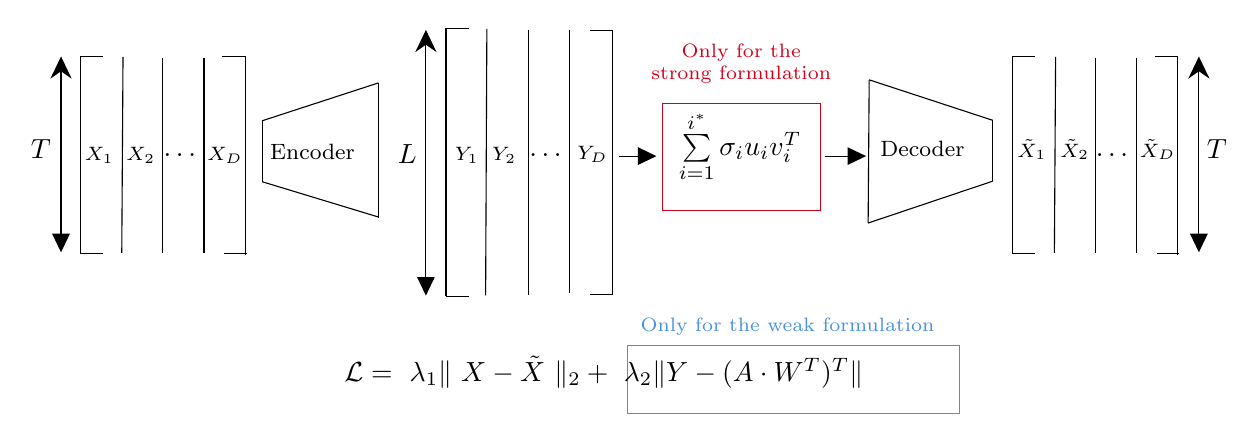
\begin{tikzpicture}[x=0.75pt,y=0.75pt,yscale=-1,xscale=1]
        %uncomment if require: \path (0,329); %set diagram left start at 0, and has height of 329

        %Straight Lines [id:da21499615368111846] 
        \draw    (37,108.56) -- (37,203.67) ;
        %Straight Lines [id:da16326946357296768] 
        \draw    (37,108.56) -- (47.89,108.56) ;
        %Straight Lines [id:da16265931324232152] 
        \draw    (37,203.67) -- (47.89,203.67) ;
        %Straight Lines [id:da5083389594267504] 
        \draw    (116.56,204.33) -- (116.56,108.67) ;
        %Straight Lines [id:da3615318503641125] 
        \draw    (117.22,203.7) -- (106.33,203.7) ;
        %Straight Lines [id:da9354769223516279] 
        \draw    (116.22,108.6) -- (105.33,108.6) ;
        %Straight Lines [id:da9284204806788381] 
        \draw    (57.67,108.87) -- (57.07,203.27) ;
        %Straight Lines [id:da9687380676381745] 
        \draw    (76.67,109.25) -- (76.67,203.25) ;
        %Straight Lines [id:da30039595434321] 
        \draw    (96.67,109.25) -- (96.67,203.25) ;
        %Straight Lines [id:da782396384119824] 
        \draw    (124.67,139.67) -- (180.67,121.42) ;
        %Straight Lines [id:da9238744798761502] 
        \draw    (124.67,169) -- (180.67,186) ;
        %Straight Lines [id:da44599235940336523] 
        \draw    (180.67,121.42) -- (180.67,186.33) ;
        %Straight Lines [id:da6964885949042201] 
        \draw    (213.3,95.06) -- (213.3,224.17) ;
        %Straight Lines [id:da06959562543054565] 
        \draw    (213.3,95.06) -- (224.19,95.06) ;
        %Straight Lines [id:da030633764479459424] 
        \draw    (213.3,224.17) -- (224.19,224.17) ;
        %Straight Lines [id:da3263511981591738] 
        \draw    (293.52,223.5) -- (293.52,96.17) ;
        %Straight Lines [id:da40502884422960217] 
        \draw    (293.52,223.5) -- (282.63,223.5) ;
        %Straight Lines [id:da8961788198500589] 
        \draw    (293.52,96.3) -- (282.63,96.3) ;
        %Straight Lines [id:da9774520960600939] 
        \draw    (232.97,95.37) -- (232.37,223.77) ;
        %Straight Lines [id:da5075505519042733] 
        \draw    (252.97,95.75) -- (252.97,223.75) ;
        %Straight Lines [id:da21045855349115494] 
        \draw    (272.97,95.75) -- (272.97,222.75) ;
        %Straight Lines [id:da754710144489299] 
        \draw    (124.67,139.67) -- (124.67,169) ;
        %Straight Lines [id:da7099185888654047] 
        \draw    (417.17,119.92) -- (476.67,139.42) ;
        %Straight Lines [id:da66143724081499] 
        \draw    (476.67,168.75) -- (416.67,188.92) ;
        %Straight Lines [id:da31064466545771574] 
        \draw    (417.17,119.92) -- (416.67,188.92) ;
        %Straight Lines [id:da5393972903258972] 
        \draw    (476.67,139.42) -- (476.67,168.75) ;
        %Straight Lines [id:da022156106633165695] 
        \draw    (296.67,156.67) -- (311.67,156.67) ;
        \draw [shift={(314.67,156.67)}, rotate = 180] [fill={rgb, 255:red, 0; green, 0; blue, 0 }  ][line width=0.08]  [draw opacity=0] (8.93,-4.29) -- (0,0) -- (8.93,4.29) -- cycle    ;
        %Straight Lines [id:da38115442380124565] 
        \draw    (395.67,156.67) -- (410.67,156.67) ;
        \draw [shift={(415.67,156.67)}, rotate = 180] [fill={rgb, 255:red, 0; green, 0; blue, 0 }  ][line width=0.08]  [draw opacity=0] (8.93,-4.29) -- (0,0) -- (8.93,4.29) -- cycle    ;
        %Shape: Rectangle [id:dp7709069667907207] 
        \draw  [color={rgb, 255:red, 208; green, 2; blue, 27 }  ,draw opacity=1 ] (317.4,131.47) -- (393.67,131.47) -- (393.67,182.67) -- (317.4,182.67) -- cycle ;
        %Shape: Rectangle [id:dp24666081940562967] 
        \draw  [color={rgb, 255:red, 74; green, 144; blue, 226 }  ,draw opacity=1 ] (300.6,248) -- (460.89,248) -- (460.89,280.67) -- (300.6,280.67) -- cycle ;
        %Straight Lines [id:da9073615867889311] 
        \draw    (27.8,111.67) -- (27.8,200) ;
        \draw [shift={(27.8,203)}, rotate = 270] [fill={rgb, 255:red, 0; green, 0; blue, 0 }  ][line width=0.08]  [draw opacity=0] (8.93,-4.29) -- (0,0) -- (8.93,4.29) -- cycle    ;
        \draw [shift={(27.8,108.67)}, rotate = 90] [fill={rgb, 255:red, 0; green, 0; blue, 0 }  ][line width=0.08]  [draw opacity=0] (10.72,-5.15) -- (0,0) -- (10.72,5.15) -- (7.12,0) -- cycle    ;
        %Straight Lines [id:da1988310735559562] 
        \draw    (203.6,98.87) -- (203.6,220.87) ;
        \draw [shift={(203.6,223.87)}, rotate = 270] [fill={rgb, 255:red, 0; green, 0; blue, 0 }  ][line width=0.08]  [draw opacity=0] (8.93,-4.29) -- (0,0) -- (8.93,4.29) -- cycle    ;
        \draw [shift={(203.6,95.87)}, rotate = 90] [fill={rgb, 255:red, 0; green, 0; blue, 0 }  ][line width=0.08]  [draw opacity=0] (10.72,-5.15) -- (0,0) -- (10.72,5.15) -- (7.12,0) -- cycle    ;
        %Straight Lines [id:da7075949415859115] 
        \draw    (486.33,108.56) -- (486.33,203.67) ;
        %Straight Lines [id:da776447423867771] 
        \draw    (486.33,108.56) -- (497.22,108.56) ;
        %Straight Lines [id:da40114415684531135] 
        \draw    (486.33,203.67) -- (497.22,203.67) ;
        %Straight Lines [id:da24114735322590564] 
        \draw    (565.89,204.33) -- (565.89,108.67) ;
        %Straight Lines [id:da8606039915940866] 
        \draw    (566.56,203.7) -- (555.67,203.7) ;
        %Straight Lines [id:da6175875067439736] 
        \draw    (565.56,108.6) -- (554.67,108.6) ;
        %Straight Lines [id:da9114789567469446] 
        \draw    (507,108.87) -- (506.4,203.27) ;
        %Straight Lines [id:da9606142652454763] 
        \draw    (526,109.25) -- (526,203.25) ;
        %Straight Lines [id:da3463806230867499] 
        \draw    (546,109.25) -- (546,203.25) ;
        %Straight Lines [id:da3635085614733373] 
        \draw    (576.02,111.67) -- (576.02,200) ;
        \draw [shift={(576.02,203)}, rotate = 270] [fill={rgb, 255:red, 0; green, 0; blue, 0 }  ][line width=0.08]  [draw opacity=0] (8.93,-4.29) -- (0,0) -- (8.93,4.29) -- cycle    ;
        \draw [shift={(576.02,108.67)}, rotate = 90] [fill={rgb, 255:red, 0; green, 0; blue, 0 }  ][line width=0.08]  [draw opacity=0] (10.72,-5.15) -- (0,0) -- (10.72,5.15) -- (7.12,0) -- cycle    ;

        % Text Node
        \draw (38,151.2) node [anchor=north west][inner sep=0.75pt]  [font=\scriptsize]  {$X_{1}$};
        % Text Node
        \draw (58,151.2) node [anchor=north west][inner sep=0.75pt]  [font=\scriptsize]  {$X_{2}$};
        % Text Node
        \draw (97,151.2) node [anchor=north west][inner sep=0.75pt]  [font=\scriptsize]  {$X_{D}$};
        % Text Node
        \draw (127.33,149.67) node [anchor=north west][inner sep=0.75pt]  [font=\footnotesize] [align=left] {Encoder};
        % Text Node
        \draw (216.3,151.23) node [anchor=north west][inner sep=0.75pt]  [font=\scriptsize]  {$Y_{1}$};
        % Text Node
        \draw (234.3,151.23) node [anchor=north west][inner sep=0.75pt]  [font=\scriptsize]  {$Y_{2}$};
        % Text Node
        \draw (275.3,150.73) node [anchor=north west][inner sep=0.75pt]  [font=\scriptsize]  {$Y_{D}$};
        % Text Node
        \draw (421.33,148.17) node [anchor=north west][inner sep=0.75pt]  [font=\footnotesize] [align=left] {Decoder};
        % Text Node
        \draw (308,101.2) node [anchor=north west][inner sep=0.75pt]  [font=\scriptsize,color={rgb, 255:red, 208; green, 2; blue, 27 }  ,opacity=1 ] [align=left] {\begin{minipage}[lt]{69.37pt}\setlength\topsep{0pt}
                \begin{center}
                    Only for the \\strong formulation
                \end{center}

            \end{minipage}};
        % Text Node
        \draw (305.8,233.2) node [anchor=north west][inner sep=0.75pt]  [font=\scriptsize,color={rgb, 255:red, 74; green, 144; blue, 226 }  ,opacity=1 ] [align=left] {Only for the weak formulation};
        % Text Node
        \draw (12,147.6) node [anchor=north west][inner sep=0.75pt]    {$T$};
        % Text Node
        \draw (188.8,149.8) node [anchor=north west][inner sep=0.75pt]    {$L$};
        % Text Node
        \draw (324.2,134) node [anchor=north west][inner sep=0.75pt]    {$\sum \limits_{i=1}^{i^{*}} \sigma _{i} u_{i} v_{i}^{T}$};
        % Text Node
        \draw (163.07,251.73) node [anchor=north west][inner sep=0.75pt]    {$\mathcal{L} =\ \lambda _{1} \| \ X-\tilde{X} \ \Vert _{2} +\ \lambda _{2} \| Y-(A\cdot W^T)^T\Vert $};
        % Text Node
        \draw (76,154.07) node [anchor=north west][inner sep=0.75pt]    {$\dotsc $};
        % Text Node
        \draw (252.13,154.07) node [anchor=north west][inner sep=0.75pt]    {$\dotsc $};
        % Text Node
        \draw (487.33,147.2) node [anchor=north west][inner sep=0.75pt]  [font=\scriptsize]  {$\tilde{X}_{1}$};
        % Text Node
        \draw (525.13,154.07) node [anchor=north west][inner sep=0.75pt]    {$\dotsc $};
        % Text Node
        \draw (508,147.2) node [anchor=north west][inner sep=0.75pt]  [font=\scriptsize]  {$\tilde{X}_{2}$};
        % Text Node
        \draw (546.33,147.2) node [anchor=north west][inner sep=0.75pt]  [font=\scriptsize]  {$\tilde{X}_{D}$};
        % Text Node
        \draw (578.56,147.6) node [anchor=north west][inner sep=0.75pt]    {$T$};


    \end{tikzpicture}

    \caption{Schematic showing the autoencoder in use as well as both methodologies. There are two terms in the loss function for the \textcolor{myblue}{Weak formulation}. On the other hand, there's an additional step before the decoder for the \textcolor{myred}{Strong formulation}.}
    \label{fig:mdoel_arch}
\end{figure}
\newpage
\begin{enumerate}
    \item \underline{The Weak formulation:} This formulation is based on \eqref{eqn:mat_form}. After choosing the number of nodes $k$, we generate two trainable matrices $A \in \mathbb{R}^{D\times k}$, and $W \in \mathbb{R}^{L\times k}$. Afterward, we reduce the number of dominant singular values of the latent space by adding a term to the loss as seen in blue in figure \ref{fig:mdoel_arch}. By doing so, we are implicitly asking the Neural Network to find the values of constants $\alpha^d_j$ and vectors $W_j$ in \eqref{eqn:alphas}, and hence imposing the latent space to be represented by the reduced basis of the chosen size (i.e. low-rank latent space). Accordingly, if training is performed properly, our trainable matrices are the basis vectors and the coefficients of the reduced basis of $Y$.

          The weak formulation finds PGD-like vectors that span the space, since we ask the Neural Network to find a basis, without enforcing the orthogonality of the vectors. Accordingly, the formulation gains some of the benefits and limitations of a PGD. On the one hand, we are finding a basis, so generalization over the test should be better since the basis should span the space of the parameters already seen in training. On the other hand, a rank that's larger than the intrinsic parametric dimension could be required to represent the entire solution.

          We will refer to this method as the Weak formulation since at the end of the training, the second term of the loss could still be large, meaning we might need more modes ($k^*>k$) to represent the latent space $Y$ correctly.

    \item \underline{The Strong formulation:} Unlike the weak formulation, this architecture enforces, in a strong manner, the dimension of the reduced basis of the latent space. Similarly to the first formulation, we choose the rank $k$ of the latent space. Then, as seen in red in figure \ref{fig:mdoel_arch}, a truncated SVD (up to the $k$th singular value) of the latent space is given to the decoder, instead of the latent space itself. Accordingly, the input of the decoder will have exactly $k$ dominant singular values. In contrast to weak formulation, we can say that the strong formulation computes a POD-like basis since the vectors are by construction orthogonal. The orthogonality of the basis vectors, as well as refraining from adding terms in the loss, should both make training and interpolating easier using this formulation.

          On the other hand, backpropagation through the singular value decomposition is not common in practice, so it could lead to unexpected behavior in some frameworks where it is not implemented correctly. Additionally, we show in Section \ref{sec:Nuemrical} that when the intrinsic parametric dimension is not given, the weak method has more flexibility to find the correct rank of the latent space, while the strong formulation only finds a good approximation of $k$.
\end{enumerate}
In both formulations, the main idea is to find a reduced basis of the latent space and enforce that the basis has a low dimension $k$. Since by the end of the training, we have the basis vectors and the coefficients, we propose to interpolate directly between the coefficients as explained in the following section.

\section{Interpolation in the latent space}\label{sec:interp}
Since both formulations previously proposed find a reduced basis of a small dimension for the latent space, we propose to interpolate between the coefficients instead of interpolating between the curves. We limit the objective of this paper to showcase the abilities of RRAEs for interpolation tasks. However, our future work will include multiple other applications such as data generation, downstream classification, and others.

What motivated us to propose this application is the limitations of linear interpolation between solutions when the solution matrix is high-rank. Take, for instance, sinusoidal curves shifted by a scalar $p$ (i.e. $\sin(x+p)$). As can be seen in figure \ref{fig:sin}, interpolating linearly between the curves corresponding to parameters $p_0 = 0$ and $p_1 = \pi$ to find the middle curve at $p^*= \pi/2$ (i.e. simply the sum divided by two) leads to the horizontal line at zero, instead of finding the correct curve shifted towards the middle.
\begin{figure}[!b]
    \centering
    \includegraphics[clip, trim=0.4cm 0cm 0cm 1cm, width=1.1\textwidth]{sin.pdf}
    \caption{Figure showing the result when interpolating linearly between two shifted sin curves, showing why linear interpolation is not a good idea for problems with multiple dominant singular values.}
    \label{fig:sin}
\end{figure}
By sending the data into a longer latent space with a low rank, we can find a simpler space where a linear interpolation would be enough to find the new curve, before going back to the original space with the decoder.

Both proposed formulations allow us to approximate the latent space by \eqref{eqn:alphas} or \eqref{eqn:mat_form}. Now say, every series of observations $X_i$ is tied to a vector of parameters $\mathbf{p}_i \in \mathbb{R}^P$. Accordingly, and since each column $W_j$ is the same for every column of Y, we can only interpolate between the coefficients $\alpha_j^d$, as we can say,
\begin{equation}
    Y_d = \sum_{j=1}^k\alpha^d_jW_j, \qquad \Longrightarrow \qquad Y(\textbf{p}_i) = \sum_{j=1}^k\gamma_j(\textbf{p}_i)W_j,
\end{equation}
where each $\gamma_j: \mathbb{R^P} \xrightarrow{} \mathbb{R}$, could be any mapping, that maps all the training parameters to the corresponding $\alpha_j^d$, and allows us to interpolate when used on new values of the parameter $p$. By that, we mean that interpolation is simply done between the coefficients inside matrix $A$ in \eqref{eqn:mat_form}.

Throughout the paper, we show that for every example presented a linear/bilinear interpolation is enough. For instance, for a parameter space of dimension one, and each $j$, we can sort the values of $\alpha_j^d$ based on their corresponding parameter values $p_i$ and write,
\begin{equation}
    \gamma_j(\mathbf{p}^*) = \gamma_j(p^*) = \alpha_m + \frac{\alpha_{m+1}-\alpha_{m}}{p_{m+1}-p_{m}}(p^*-p_{m}).
\end{equation}
where we distinguish between the \textbf{bold} notation for vectors and non-bold for scalars, $m$ is the index of the largest value of $p$ that is smaller than $p^*$, and both $p_0 = \alpha_0 =0$ for the equation to be valid for any $i\in[1, d]$.

Similarly, bilinear interpolation is performed between the four closest values of $\alpha_j^d$ from the top right, top left, bottom right, and bottom left respectively (for details, refer to the Appendix).

Finally, for higher dimensional cases, more elaborated techniques could be used for interpolation (e.g. the sPGD), or even a Neural Network. Yet, the drawback of using a Neural Network is that we would need a Neural Network for every mapping $\gamma_j$. In other words, $k$ Neural Networks to train! As we show throughout the paper, interpolating linearly/bilinearly between the coefficients is good enough since the Autoencoder already did the linearization. However, interested readers can find some of our results using $k$ trainable Neural Networks in the Appendix as well.
\section{Insights behind RRAEs}\label{sec:insights}
Autoencoders were originally introduced with smaller latent dimensions for feature recognition and data reduction. Overall, Vanilla autoencoders try to find only a few features that represent the data before giving these back to the decoder. The papers that presented the IRMAE \cite{jing2020implicit}, and LoRAE \cite{mazumder2023learning} provided many examples showing that longer low-rank latent spaces lead to better results in interpolation, data generation, and downstream classification. However, the reasons behind the success of longer low-rank latent spaces are not clarified. In this section, we provide two arguments that explain why a long latent space of rank $k$ can lead to better training/interpolation than a latent space of length $k$. Specifically, we argue that finding a basis for the low-rank latent space leads to much better interpolations. We give our opinion on the validity of the arguments presented and provide two examples to support our claims.

\underline{1- Longer latent spaces lead to more flexibility in encoding:} As has been shown in many applications (e.g. Koopman Theory), a larger dimension leads to more linear behavior. Accordingly, by enlarging the latent space and asking the Neural Network to only use a reduced version of the matrix (i.e. both our Weak and Strong formulations), we allow the encoder to find more linear embeddings in the latent space, to then choose a few of them. Accordingly, for the same training parameters, while a regular autoencoder might find highly nonlinear coefficients to fit the training data, RRAEs tend to find more ``linear'' ones. Even though both could lead to great results on the training data, when interpolating (especially linearly in the latent space), Vanilla Autoencoders won't have the same generalization capabilities as RRAEs. Additionally, by finding a basis of the latent space, RRAEs should be able to generalize better over the test data, since the basis should span the space of the parameters already seen in training, whether with a POD-like basis (the strong formulation), or a PGD-like one (the weak formulation). The Vanilla Autoencoder on the other hand has holes in its interpolation \cite{jing2020implicit}, since it does not find a basis, but only coefficients that are helpful for the decoder to retrieve the solution.

\underline{2- Longer latent spaces are easier to decode:} A long latent matrix of rank $k$ includes exactly as much information as a matrix of length $k$ with full rank. In other words, the decoder does not receive any more information when longer, but low-rank latent spaces are used. However, decoding with much longer latent spaces is easier since duplicated data is given to the network. For instance when $k=1$, a Vanilla autoencoder's latent space will contain only a constant per solution (say $c_i$). However, a longer latent space would include linear combinations as $\alpha_lc_i$ where $l \in [1, L]$. So the bigger the latent space, the more duplicated data is given to the decoder which can help it in untangling the relationships between parameters. Since the information given is the same, we believe that a powerful decoder (e.g. many layers) should be able to reconstruct the data even in a Vanilla autoencoder. In other words, smaller decoders can be used with RRAEs, and in complicated examples (e.g. pictures with multiple parameters, or curves that intersect multiple times), RRAEs can have better results, even over the training data.

To explore further the arguments presented above, we test Vanilla Autoencoders and both our formulations on two examples characterized by one parameter. The first curves we propose are shifted sin curves since these have a simple nonlinearity, but they are hard to separate (nonmonotonic and cross each other multiple times). The second example we chose is curves with stair-like behavior. In this example, we create highly nonlinear curves (different supports, different numbers of jumps, etc.), but we define them to be monotonic and only cross each other occasionally (i.e. easier to separate). The equations used to define the columns of our input matrix $X$ in each case are as follows,
\begin{equation}
    \begin{cases}
        X_d(t_v,\, p_d) = f_{shift}(t_v, \, p_d) = \sin(t_v-p_d\pi), \hspace{0.1cm}\qquad\quad & p_d \in [0, 1.5], \\[1.2ex]
        X_d(t_v, \,p_d) = f_{stair}(t_v,\, p_d, \, \text{args}) \qquad\quad                    & p_d \in [1, 5],
    \end{cases}
\end{equation}
where $t_v \in \mathbb{R}^T$ is a vector of time at which observations are done, and $f_{stair}$ takes some arguments ``args'' as detailed in the following algorithm,\\[2ex]
\begin{algorithm}[H]
    \SetKwInput{Input}{Input}
    \SetKwInput{Output}{Output}

    \Input{$p_d\in \mathbb{R}$, $t_v \in \mathbb{R}^T, (\text{Ph}_0, \text{Amp}_0,\kappa, y_0, w) \in \mathbb{R}$}
    ~\\
    $\text{Amp}_{p_d} = p_d$\\[1.6ex]
    $\displaystyle\text{Ph}_{p_d} = \text{Ph}_0+\kappa(\text{Amp}_{p_d}-\text{Amp}_0)$\\[1.6ex]
    $g_{p_d}(t_v) = \text{Amp}_{p_d}\sqrt{t_v}\sin(w(t_v-\text{Ph}_{p_d}))-y_0$\\[1.6ex]
    $\displaystyle h_{p_d}(t) = \left(\frac{\left|g_{p_d}(t)\right|+g_{p_d}(t)}{2}\right)^5$\\[1.6ex]
    $X_d(t_v, \, p_d)=\text{cumsum}(h_{p_d}(t_v))$
    ~\\
    ~\\
    \Output{$X_d(t_v, \, p_d)$ for each parameter $p_d$.}
    \caption{Algorithm to find $f_{stair}$ for a list of parameters $\textbf{p}$.}
\end{algorithm}
In this paper, we choose the initial parameters of the stair function to be,
\begin{equation}
    \begin{cases}
        \text{Ph}_0 = 0.875, \qquad \text{Amp}_0=1 \\
        \kappa = 2.286, \qquad y_0 = 2.3, \qquad w = 2\pi.
    \end{cases}
\end{equation}
Training is performed over 14, and 35 equidistant values of $p_d$ for the shifted $\sin$ curves and the stair-like curves respectively. We then test on 20 and 100 random values of $p_d$, respectively, chosen inside the training domain. The large number of tests is to guarantee that the models are learning the dynamics and not just the training curves and some tests nearby. Since the solution curves depend on one parameter, we use a Vanilla Autoencoder with a scalar latent space and an RRAE with a longer latent space of rank one. As detailed in \textcolor{red}{Appendix A}, we fix every other training parameter to ensure a fair comparison. The relative error over all $p_d$ values for both the train and test sets is documented in the following table,
\begin{table}[!h]
    \centering
    \begin{tabular}{|c|c|c|c|c|}
        \hhline{~|----|}
        \multicolumn{1}{c|}{} & \multicolumn{2}{c|}{Shifted sin} & \multicolumn{2}{c|}{Stair-like}                                \\
        \hhline{~|----|}
        \multicolumn{1}{c|}{} & Train Error                      & Test Error                      & Train Error   & Test Error   \\
        \hline
        Vanilla AE            & 2.46                             & 31.26                           & 2.97          & 3.74         \\
        \hline
        RRAE (Strong)         & \textbf{1.35}                    & \textbf{2.4}                    & \textbf{1.87} & \textbf{3.2} \\
        \hline
        RRAE (Weak)           & 3.71                             & 7.3                             & 4.11          & 5.76         \\
        \hline
    \end{tabular}
    \caption{Table showing the relative error (in \%) for all three architectures on both the train and test set for both the examples of shifted sin curves and stair-like ones.}
    \label{fig:table_shift_sin}
\end{table}

The results presented in the table depict the arguments presented above and some of their limitations. First of all, we can see that the Vanilla Autoencoder is overfitting the data when trained over the shifted $sin$ functions. Since these are very hard to separate, and as mentioned in the first argument before, the Vanilla autoencoder is simply converging to coefficients that fit the training data, but are not generalizable. On the other hand, the RRAEs with both formulations are doing much better on the test set, with the strong formulation achieving better results than the weak one. When comparing the formulations to the POD and the PGD, we expect, that for the same rank in the latent space that is equal to the dimension of the parametric space, the PGD basis wouldn't be as efficient as the one found by the POD.

Additionally, the results on the train set show that the strong formulation is doing better than the Vanilla Autoencoder, even though the Vanilla AE is freeier to find more nonlinear coefficients. This illustrates what we proposed in the second argument, since for the same decoder size, the RRAE can fit better the training data. But is what's proposed true for every curve?

Opposingly, the results on the stair-like curves show that if the curves are highly nonlinear but easily separable (in this case, monotonic curves with little intersections between them), the Vanilla Autoencoder can fit both the train and test data well. Again, the strong formulation can fit the training data better, showing one more time that the duplicated values in the latent space help the training set. The weak formulation is as expected, doing worse than the strong one with the same rank in the latent space. However, the low error of the Vanilla AE on the test set shows that, when curves can easily be separated, the classical AE can do almost as well as the strong formulation, and even better than the weak one.

The results of these two examples explain why RRAEs can be much better than Vanilla Autoencoders for interpolation tasks. These also show that on very simple curves with one parameter, the effect of longer latent spaces is reduced. As clearly shown in all the other examples in Section \ref{sec:Nuemrical}, and as observed for pictures with multiple parameters in \cite{jing2020implicit} and \cite{mazumder2023learning}, choosing a longer latent space with a low rank provides much better results on larger parametric spaces and more complicated curves.

To further understand the significance of the results, we depict the predictions of all three architectures over both examples in figure \ref{fig:sin_shift_test}.
\begin{figure}[!b]
    \centering
    \includegraphics[clip, scale=0.38, trim=3cm 1cm 0cm 2cm]{sin_shift_plot_test.pdf}
    \caption{Figure showing the predictions of Vanilla Autoencoders and RRAEs with both formulations over two particular values of $p_d$ for the shifted $sin$ and stair-like examples.}
    \label{fig:sin_shift_test}
\end{figure}
We chose on purpose two values of $p_d$ that were the hardest to interpolate for all techniques. As can be seen in the figure, The Vanilla Autoencoder's predictions (in blue) are much worse than RRAEs with both formulations for the shifted sin curve with $p_d=0.94$. On the other hand, it is interesting that the weak formulation is doing as bad as the Vanilla AE for a very small value of $p_d$ (top left of the figure). A closer look at the interpolation error of the weak formulation shows that it interpolates as well as the strong formulation over every value of $p_d$ except for very small ones. On the stair-like function though, all three formulations have almost the same interpolation capabilities over most tests.

To explain this behavior and strengthen the arguments we provided at the beginning of the section, we plot the latent space coefficients in figure \ref{fig:sin_shift_latent}. It is important to note that the coefficients are defined differently between the RRAE and the Vanilla AE. On the one hand, we remind the reader that the latent space for RRAEs can be written as in \eqref{eqn:mat_form}. However, since we enforce a rank of $1$ in this example, $A \in \mathbb{R}^D$ is simply a vector of coefficients (one for each curve, between which we interpolate). Figure \ref{fig:sin_shift_latent} shows the values inside vector $A$ plotted against the corresponding parameters for both the weak and strong formulations. On the other hand, since the latent space of the Vanilla autoencoder is of length one, its latent space is only a constant per curve (again, between which we interpolate) and hence we draw the latent space against the corresponding parameters for the Vanilla AE.
\begin{figure}[!b]
    \centering
    \includegraphics[clip, scale=0.38, trim=2.9cm 1cm 0cm 1.5cm]{sin_shift_plot_latent.pdf}
    \caption{Figure showing the coefficients to be interpolated (dots) for all three architectures, and the interpolated values for the test set (crosses).}
    \label{fig:sin_shift_latent}
\end{figure}

The coefficients show why both the weak and the strong formulations have better interpolation capabilities. The main problem with the coefficients found by the Vanilla AE for the shifted sin curves (the blue crosses and dots to the left) is that the resulting curve from linearly interpolating the coefficients is not an injection, over most of the domain. Specifically, looking between the vertical black dashed lines, any value of $p$ (say $p_1=1.1$) will have the same coefficient as another $p$ nearby ($p_2$ around 1.25). Accordingly, the decoder will find the same curve for two different parameters, which is wrong since $p$ defines a shift. The same thing can be said about another interval from $p=0$ to around $p=0.3$. This reasoning explains why the Vanilla AE isn't capable of interpolating between the sin curves, but why are both the weak/strong formulations doing better?

Based on the first argument proposed earlier in this section, a longer latent space allows RRAEs to find more ``linear" coefficients. This is clearly shown by the coefficients of the strong method (in green, to the left) which have a linear monotonic behavior. On the other hand, the weak formulation finds monotonic coefficients in the range $p\in[0.2, 1.4]$ but has the same problem as the Vanilla AE when $p\in[0, 0.2]$. Accordingly, the RRAE with the weak formulation can interpolate on most of the domain except a small part in the beginning. This explains why the weak formulation is doing as bad as the Vanilla AE on $p=0.06$, and why its relative error over all the test curves is much lower than Vanilla Autoencoder.

Finally, when looking at the coefficients for the stair-like problem (to the right of figure \ref{fig:sin_shift_latent}), we can see that since the curves are easily separable, the Vanilla AE can find monotonic coefficients, which explains why it can interpolate well in this example. It is important to note here that we talk about ``monotonic'' coefficients since we only have one parameter. Over parametric domains of higher dimensions, RRAEs are building a basis and will hence have a much bigger advantage over Vanilla AEs, as shown in many examples in section \ref{sec:Nuemrical}.

Overall, our results over those two simple examples show how duplicated data benefits RRAEs, and hence why we can use smaller decoders to achieve the same result (argument 2). In addition, we showed how increasing the dimension of the latent space helps the Autoencoder to find more linear coefficients, leading to better interpolation results (argument 1). Both our examples were with one parameter, where the advantage of building a basis is limited (since the basis in this case is just a vector). As we show in the following sections, over curves with parametric spaces of dimension two for instance, creating a basis for long low-rank latent spaces leads to much better interpolations than Vanilla Autoencoders. This is expected since if the training set is big enough, the basis found by the RRAEs will span the whole parametric space.

\section{Testing on Numerical Data}\label{sec:Nuemrical}
In this section, we use RRAEs to interpolate between curves with high-rank solution matrices. Our results show that RRAEs with both formulations can interpolate between curves with one/two parameters even if a linear/bilinear interpolation is used in the latent space. We also show how using a POD before the RRAE can filter noisy data and limit the computational overhead for long time series (i.e. when $T$ in figure \ref{fig:mdoel_arch} is large). Finally, we illustrate how RRAEs can find the dimension of the parametric space (or a close approximation) by themselves if a random larger rank of the latent space is chosen.
\subsection{Examples with one/two parameters}\label{sec:numerical_example}
In this subsection, we test the robustness of our proposed formulations over three problems. First, we choose accelerated sin curves, which are again parametrized by one parameter, but much harder to learn than shifted curves. We then propose two examples characterized by two parameters; first, the sum of two sin curves with different frequencies, as well as two gausses in two different locations. We show how in such examples, Vanilla Autoencoders are not able to interpolate, and that both our formulations have much better results for the same training parameters (again, training details can be found in Appendix \textcolor{red}{AAA}). We define the columns of our input matrix $X_d(t_v,\, p_d) = f_{prob}$ for each problem as follows,
\begin{equation}\nonumber
    \begin{cases}
        f_{acc}(t_v, \, p_d) = \sin(p_dt_v), \hspace{0.1cm}\qquad\quad                                                                                  & p_d \in [0, 1.5],                         \\[1.2ex]
        f_{freqs}(t_v,\, \textbf{p}_d) = \sin(p^1_dt_v)+\sin(p^2_dt_v) \qquad\quad                                                                      & p^1_d \in [1, 5], \quad p^2_d \in [1, 5], \\[1.5ex]
        f_{gauss}(t_v,\, \textbf{p}_d) =  1.3e^{\displaystyle -\frac{(t_v-p^1_d)^2}{0.08}}+1.3e^{\displaystyle -\frac{(t_v-p^2_d)^2}{0.08}} \qquad\quad & p^1_d \in [1, 5], \quad p^2_d \in [1, 5],
    \end{cases}
\end{equation}
Where again, we distinguish between the \textbf{bold} notation for vectors and non-bold ones for scalars. In both the second and third expressions, our parametric space is of dimension $2$ and so $\textbf{p}_d = [p^1_d, \,p^2_d] \in \mathbb{R}^2$. Again, we only use linear/bilinear interpolation in the latent space, since the RRAEs should have dealt with the nonlinearity already. The results on two interpolated curves over each example for all three formulations can be seen in figure \ref{fig:sin_sin_gauss}.
\begin{figure}[!h]
    \centering
    \includegraphics[clip, scale=0.38, trim=3.6cm 1cm 0cm 1.5cm]{sin_sin_gauss_plot_test.pdf}
    \caption{Figure showing the interpolated results of RRAEs with both formulations, as well as a Vanilla AE on the three examples presented with linear/bilinear interpolation in the latent space.}
    \label{fig:sin_sin_gauss}
\end{figure}

We also present the relative error over all the training/test sets in the following table,
\begin{table}[!h]
    \centering
    \begin{tabular}{|c|c|c|c|c|c|c|}
        \hhline{~|------|}
        \multicolumn{1}{c|}{} & \multicolumn{2}{c|}{\hspace{0.15cm} Accelerated sin\hspace{0.15cm} } & \multicolumn{2}{c|}{Mult. Frequencies} & \multicolumn{2}{c|}{\hspace{0.1cm} Mult. Gausses\hspace{0.1cm} }                                                                          \\
        \hhline{~|------|}
        \multicolumn{1}{c|}{} & \hspace{0.08cm} Train    \hspace{0.08cm}                             & Test                                   & \hspace{0.08cm} Train \hspace{0.08cm}                            & Test          & \hspace{0.08cm}  Train\hspace{0.08cm} & Test           \\
        \hline
        Vanilla AE            & 50.57                                                                & 52.19                                  & 11.74                                                            & 17.72         & 16.41                                 & 31.32          \\
        \hline
        RRAE (Strong)         & \textbf{3.2}                                                         & \textbf{3.13}                          & \textbf{4.7}                                                     & \textbf{9.68} & \textbf{8.67}                         & \textbf{14.67} \\
        \hline
        RRAE (Weak)           & 9.41                                                                 & 8.62                                   & 13.94                                                            & 15.55         & 15.31                                 & 20.99          \\
        \hline
    \end{tabular}
    \caption{Table showing the relative error (in \%) for all three architectures on both the train and test set for the three examples with one/two parameters.}
    \label{fig:table_sin_sin_gauss}
\end{table}
As can be seen in both the table and the figures, RRAEs with both formulations can interpolate much better than Vanilla AEs when linear/bilinear interpolation is used. Again, the weak formulation is not doing as well as the strong one for the same rank of the latent space which is expected. Most importantly, RRAEs can interpolate between curves with high-rank solutions, even those with different supports (i.e. the multiple gausses). We hope that from the previous section, we gave enough evidence to explain why RRAEs are much better at interpolation than regular AEs, especially with multiple parameters since a reduced basis is found.
\subsection{Extensions of RRAES}\label{sec:extensions}
From the results already presented, it is clear that RRAEs have a lot of potential when it comes to interpolation. However, readers might be wondering, what if I don't know the dimension of the parametric space? On the other hand, since Neural Networks do not discriminate between the dynamics and noise, won't noise be linearised with the data as well? And what if the time series is long (i.e. $T \gg 1$), won't the training take too much time? In the following section, we answer all of these questions by showing that RRAEs can conclude by themselves an approximate dimension of the parametric space, and combining a POD with the proposed model can filter noise and limit the computational overhead. To do so, we choose to interpolate between curves representing crystallization rates, governed by the Avrami equation as follows,
\begin{equation}
    X_d(t_v, \, \mathbf{p}_d) = 1-e^{\displaystyle -\frac{\pi p^1_d\left(p^2_d\right)^3}{3}t_v^4}, \qquad p^1_d \in [1.5, 3], \qquad p^2_d \in [1.5, 3].
\end{equation}
\begin{figure}[!b]
    \centering
    \includegraphics[clip, scale=0.38, trim=3.1cm 1cm 0cm 1.5cm]{avrami_ww_noise_test.pdf}
    \caption{Figure showing the interpolated results of RRAEs with both formulations, as well as a Vanilla AE on the crystallization rates with different latent space dimensions and with/without noise.}
    \label{fig:crystallization}
\end{figure}
Here our parameters $p^1_d$ and $p^2_d$ represent the nucleation rate per unit volume and the growth velocity respectively. Again, for details about the chosen parameters for train/test sets, readers are referred to \textcolor{red}{Appendix A}. To check whether RRAEs can determine the parametric dimension by themselves, we train the model with a latent space of rank $2$ (the original dimension of the parametric space), $3$, $5$, and $10$. On the other hand, to show that the model can filter noise, we add random Gaussian noise to the data and train the model combined with a POD. Mainly, the idea is to reduce the dimension of the input matrix $X$ with a POD, and then perform training over the reduced data before going back to the original data by applying the inverse transformation to the output of the decoder. The results for some of the interpolated curves can be seen in figure \ref{fig:crystallization}.

To have clearer figures, we only plot the result for training with a latent space of rank $10$ (i.e. ``Strong-10", and ``Weak 10") since these must struggle the most in finding the intrinsic dimension of the parametric space. Similarly, we only plot two random curves for each of the strong/weak formulations used with a POD (i.e. ``POD-strong'', and ``POD-weak'').

As can be clearly shown to the right of the figure, the combination of a POD with an RRAE can filter noise to find smoother curves. Since the POD reduces the dimension, this leads to significantly smaller computational overheads. For example, training was done over a dimension $T_{POD} = 4$ instead of the original $T = 300$.

To be able to properly compare between the different ranks of the latent spaces, we present the relative error for each training in the table below,

\begin{table}[!h]
    \centering
    \begin{tabular}{|c|c|c|c|c|}
        \hhline{~|----|}
        \multicolumn{1}{c|}{} & \multicolumn{2}{c|}{Weak formulation }   & \multicolumn{2}{c|}{Strong Formulation}                                                \\
        \hline
        Rank                  & \hspace{0.08cm} Train    \hspace{0.08cm} & Test                                    & \hspace{0.08cm} Train \hspace{0.08cm} & Test \\
        \hline
        2                     & 0.65                                     & 3.38                                    & 0.36                                  & 1.81 \\
        \hline
        3                     & 0.81                                     & 1.97                                    & 0.35                                  & 1.81 \\
        \hline
        5                     & 0.59                                     & 1.85                                    & 0.41                                  & 1.84 \\
        \hline
        10                    & 0.62                                     & 1.99                                    & 0.68                                  & 1.9  \\
        \hline
    \end{tabular}
    \caption{Table showing the relative error (in \%) when different ranks are enforced for the latent space to learn interpolation over the crystallization rates.}
    \label{fig:table_avramis}
\end{table}
The results documented in the table, as well as the two curves plotted to the left of figure \ref{fig:crystallization}, show that specifying a rank for the latent space that's different than the intrinsic dimension doesn't affect the results on the test set by much. What's also interesting is that the results for the weak formulation are better when the rank specified is bigger than $2$ (the dimension of the parametric space). Again, by comparing the Weak formulation with a PGD, it is expected that the Neural Network can converge to basis vectors that are not orthogonal and hence might need a larger rank (i.e. a larger dimension of the basis) to represent the data best.

Finally, the remaining question is whether those good results are caused by the RRAEs finding the intrinsic dimension, or if they are capable of representing properly a space of dimension two with a basis of dimensions $3$, $5$, and $10$. Accordingly, we plot the first five singular values (normalized) of the latent space in figure \ref{fig:sing_vals_avrami}.
\begin{figure}[!t]
    \centering
    \includegraphics[clip, scale=0.38, trim=3.6cm 1cm 0cm 1.5cm]{avrami_ww_noise_sv.pdf}
    \caption{Figure showing the first five singular values of the latent spaced normalized when different ranks of the latent space are enforced with the weak (left) and the strong (right) formulations.}
    \label{fig:sing_vals_avrami}
\end{figure}
In the figure, the blue curve has only two dominant modes, since we enforce the latent space to have a rank of $2$. But what's interesting is that no matter how big we choose the rank of the latent space to be, both formulations learn automatically to only use a small rank! Since by using the weak formulation, we allow the Neural Network to directly modify the coefficients, we can see that in all cases, the RRAE finds exactly the intrinsic dimension $2$, since the singular values of the latent space are much smaller from the third one onwards. On the other hand, the strong formulation is only able to find an approximation of the intrinsic dimension, since it uses approximately a rank 3 in all the cases where $k>2$. However, as can be seen in table \ref{fig:table_avramis}, the strong formulation was able to find a basis that represents the whole data even with an additional dimension. In both cases, we show in this example that RRAEs can find an approximation of the dimension of the parametric space by themselves, and hence not knowing the dimension beforehand is not a problem when using these architectures.
\section{Summary and Conclusions}\label{sec:conclusions}
In this article, we presented Rank Reduction Autoencoders (RRAEs), Autoencoders that enforce a reduced basis of long latent spaces. We proposed two formulations, the strong formulation which finds a reduced basis that's POD-like, and a weak formulation that forms a PGD-like basis. We also propose to interpolate linearly between the coefficients of the basis instead of the curves in the latent space.

We provided multiple reasons why longer latent spaces with low rank can be much more effective than reduced latent space, and we backed up our arguments with two simple examples.

We tested RRAEs on examples characterized by one/two parameters and showed that both formulations can interpolate well between curves that formed originally a high-rank matrix when the rank of the latent space is enforced to be equal to the dimension of the original parametric space.

Finally, we showed how RRAEs can filter noise and have much less computational overhead when combined with a POD. We also provided an example that showed that not knowing the dimension of the parametric space in advance won't significantly affect the interpolation of RRAEs. In other words, they can find an approximation of the intrinsic dimension by themselves.

All in all, our results show that Rank Reduction autoencoders have a huge potential when it comes to interpolation over nonlinear manifolds. The strong formulation provides the best results on train/test data, and the weak formulation can find a better approximation of the intrinsic dimension of the parametric space if it is unknown in advance.

Readers who are interested in testing the autoencoders for themselves can find our code on our \href{https://gitfront.io/r/jadm133/fvL5vzbqqGLB/RRAEs/}{GitHub repository}, done in \texttt{JAX}. For any questions and concerns, feel free to reach us there as well.

%%=============================================%%
%% For submissions to Nature Portfolio Journals %%
%% please use the heading ``Extended Data''.   %%
%%=============================================%%

%%=============================================================%%
%% Sample for another appendix section			       %%
%%=============================================================%%

%% \section{Example of another appendix section}\label{secA2}%
%% Appendices may be used for helpful, supporting or essential material that would otherwise 
%% clutter, break up or be distracting to the text. Appendices can consist of sections, figures, 
%% tables and equations etc.





\newpage
\bibliographystyle{unsrt}
%\bibliographystyle{apalike}

\bibliography{sn-bibliography}
\newpage
\section*{Appendix}
Before introducing the testing examples, we begin by explaining our logic behind the choice of the autoencoder architecture, which we believe should be considered a logical choice for almost any input. These include the following:
\begin{enumerate}
    \item The encoder: As previously mentioned, the encoder is chosen to be an MLP. We believe that the number of layers and Neurons for the encoder should be small. The main reason is that the decoder has to find the inverse function, which becomes much more complicated the larger the encoding network is. For this article, we choose an encoder of depth 1 (one hidden layer), and width 20 (20 Neurons).
    \item The decoder: Since the decoder has to find inverse maps, we use deeper MLPs. For both proposed formulations, we find that a decoder with either 4 hidden layers and 64 Neurons for each layer is usually enough to be able to decode the latent space.
    \item The latent space dimension $L$: Autoencoders give us the choice of the dimension $L$, which could be either bigger or smaller than the original dimension $T$. However, the shorter the latent space, the harder it is for the decoder to find the inverse map. On the other hand, the longer the latent space, the more the decoder's prediction is affected by the errors in the latent space. For instance, an error of $1\%$ over 5 values has less effect on the decoder results than an error of $1\%$ over 50 values. Since we chose the decoder to be a deeper Neural Network, we decided to reduce the dimension space, hoping that the decoder would be able to find the prediction even while using only a few values. For this article, we find $L$ by multiplying the time dimension $T$ by $0.2$ and rounding to the nearest integer.
    \item The loss weights: We chose all the weights in the loss to be equal to one. We believe that with the good choice of the architecture presented above, changing the constants won't be necessary.
    \item Other training parameters: To show the flexibility and rigidity of our model, we choose almost fixed training parameters. We don't try to fine-tune these to get better results. The purpose of doing so is to show how powerful the RRAE is, and that with all the carefully selected parameters above, it can achieve small errors even for complicated examples. We perform 4 training loops, each of $2900$ epochs, and a learning rate that's reduced from 1e-3 to 1e-6 by dividing by ten. Even though the number of epochs appears to be large, most epochs are not reached because we enforce a strong stagnation condition that stops the loops when the error stops decreasing. In addition, we used batches with sizes that range from $4$ to $16$, depending on the total number of curves and the formulation. In general, a larger batch size was required by the Weak formulation to converge.
\end{enumerate}

\underline{Note for training:} Since in \eqref{eqn:alphas}, the constants $\alpha$ can be anything, but the vectors $W_j$ are normalized, we normalize each column of matrix $W$ after every gradient descent. In addition, our initial guess of $A$ and $W$ is normalized, so we use a bigger learning rate for those matrices compared to the rest of the Neural Network. The main reason is to allow the Neural Network to change significantly the values of the coefficients $\alpha_j^d$ even if the rest of the Neural Network doesn't need/can't sustain larger learning rates (more details in Section \textcolor{red}{AAA}).

\end{document}